\documentclass[10pt, hyperref={bookmarks=true}, aspectratio=169]{beamer}
\usepackage[utf8]{luainputenc}
\usepackage{polyglossia}
\setdefaultlanguage{russian}
\setotherlanguage{english}

\usetheme[minimal]{RUDN}

%\setbeamertemplate{footline}[frame number]

%%%%%%%%%%%%%%%%%%%%%%%%%%%%%%%%%%%%%%%%%%%%%%%%%%%%%%%%%%%%%%%%%%%%%%%%%%%%%%%%
%% Настройки титульного слайда
%%%%%%%%%%%%%%%%%%%%%%%%%%%%%%%%%%%%%%%%%%%%%%%%%%%%%%%%%%%%%%%%%%%%%%%%%%%%%%%%
\title[Стиль презентации для РУДН]{\textbf{Стиль презентации для РУДН}}

\subtitle[Подзаголовок]{Подзаголовок}

\author[Александр Захаров]{Александр Захаров\inst{\tiny 1} \and Ещё автор\inst{\tiny 2}}

\institute[РУДН]{
  \inst{1}
  Математический институт им. Никольского\\
  ФФМиЕН, РУДН.
  \and
  \inst{2}
  Смехатический хохмститут им. Никулина\\
  КеК, ЛОЛ.
}

\date[МКК, 2025-04-01]{Международная конференция конференций\\ 1 Апреля, 2025гг.}
%%%%%%%%%%%%%%%%%%%%%%%%%%%%%%%%%%%%%%%%%%%%%%%%%%%%%%%%%%%%%%%%%%%%%%%%%%%%%%%%

%% Уберите или добавьте комментарии к строкам ниже, если хотите включить/выключить
%% повторный показ слайда с содержанием перед каждой новой главой презентации.

\AtBeginSection[]
{
  \begin{frame}
    \frametitle{Содержание - текущая секция}
    \tableofcontents[currentsection]
  \end{frame}
}

%%%%%%%%%%%%%%%%%%%%%%%%%%%%%%%%%%%%%%%%%%%%%%%%%%%%%%%%%%%%%%%%%%%%%%%%%%%%%%%%


\begin{document}

\frame{\titlepage}

%%%%%%%%%%%%%%%%%%%%%%%%%%%%%%%%%%%%%%%%%%%%%%%%%%%%%%%%%%%%%%%%%%%%%%%%%%%%%%%%

\begin{frame}
\frametitle{Содержание}
\tableofcontents
\end{frame}

%%%%%%%%%%%%%%%%%%%%%%%%%%%%%%%%%%%%%%%%%%%%%%%%%%%%%%%%%%%%%%%%%%%%%%%%%%%%%%%%

\section{Как работать с появлением текста на слайде}

%%%%%%%%%%%%%%%%%%%%%%%%%%%%%%%%%%%%%%%%%%%%%%%%%%%%%%%%%%%%%%%%%%%%%%%%%%%%%%%%

\begin{frame}
\frametitle{Пример обычного слайда с поэтапным списком}

Мы вынуждены отталкиваться от того, что убеждённость некоторых оппонентов требует от нас анализа позиций, занимаемых участниками в отношении поставленных задач.

\begin{itemize}
\item<1-> Список 1
\item<2-> Список 2
\item<3-> Список 3
\end{itemize}

\end{frame}

%%%%%%%%%%%%%%%%%%%%%%%%%%%%%%%%%%%%%%%%%%%%%%%%%%%%%%%%%%%%%%%%%%%%%%%%%%%%%%%%

\begin{frame}
  \frametitle{Как использовать команду \texttt{\textbackslash{pause}}}
  Например, я ввёл этот текст и добавил \texttt{\textbackslash pause}, \pause

  теперь этот текст и формулы появятся только на следующем слайде
  \begin{align*}
    f(x) &= x^2\\
    g(x) &= \frac{1}{x}\\
    F(x) &= \int^a_b \frac{1}{3}x^3
  \end{align*}

  \pause

  а этот текст и того позднее.
\end{frame}



%%%%%%%%%%%%%%%%%%%%%%%%%%%%%%%%%%%%%%%%%%%%%%%%%%%%%%%%%%%%%%%%%%%%%%%%%%%%%%%%

\section{Выделение текста}

%%%%%%%%%%%%%%%%%%%%%%%%%%%%%%%%%%%%%%%%%%%%%%%%%%%%%%%%%%%%%%%%%%%%%%%%%%%%%%%%


\begin{frame}
\frametitle{Выделение текста}

Вот так можно обратить внимание слушателей \alert{на текст командой \texttt{\textbackslash alert}}.

\begin{block}{Люблю грозу в начале мая,}
  Когда весенний, первый гром,
\end{block}

\begin{alertblock}{Как бы резвяся}
  и играя,
\end{alertblock}

\begin{examples}
  Грохочет в небе голубом.
\end{examples}

\end{frame}
%%%%%%%%%%%%%%%%%%%%%%%%%%%%%%%%%%%%%%%%%%%%%%%%%%%%%%%%%%%%%%%%%%%%%%%%%%%%%%%%

\begin{frame}
\frametitle{Текст в две колонки с картинкой}

\begin{columns}

\column{0.45\textwidth}

\begin{figure}
    \centering
    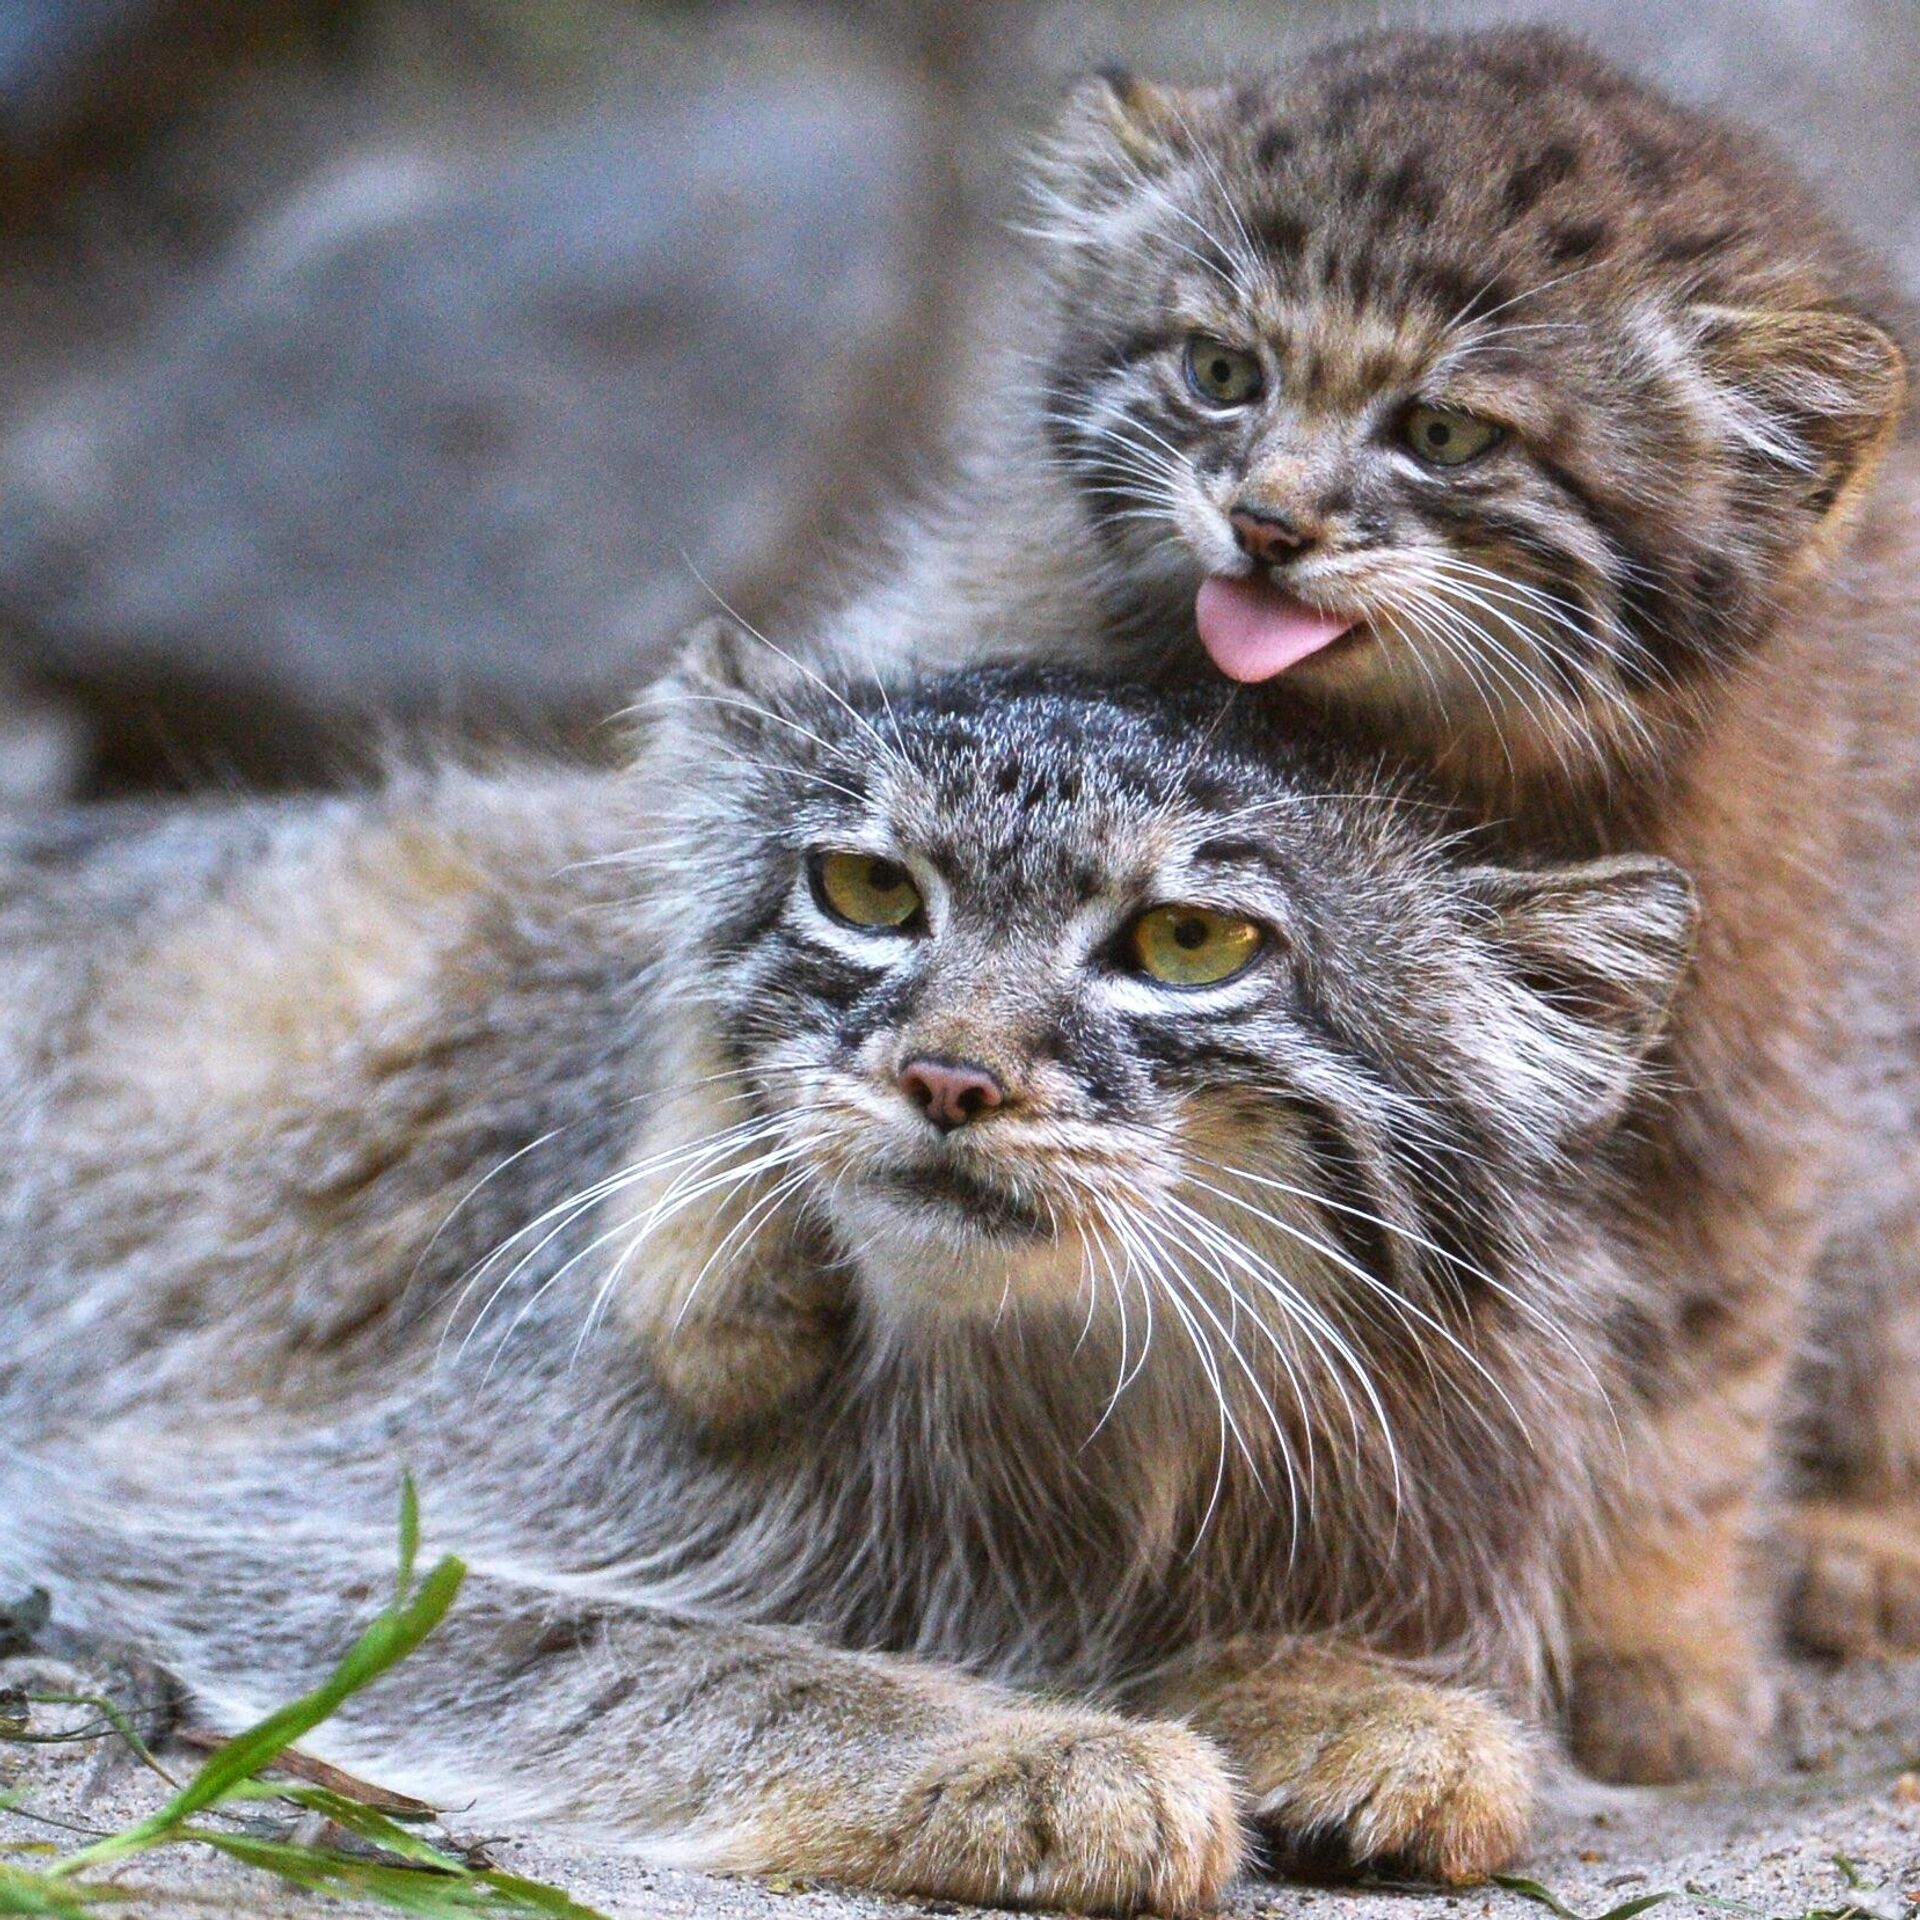
\includegraphics[width=\columnwidth]{./img/manuls.jpg}
    \caption{{Котята манулов} \newline \tiny{(Загружено c https://ria.ru/20201208/manul-1588107027.html)}}
    \label{картинка:котята-манулов}
\end{figure}


\column{0.55\textwidth}
А это текст во второй колонке!

\texttt{\textbackslash (0o0)/}

\end{columns}
\end{frame}

%%%%%%%%%%%%%%%%%%%%%%%%%%%%%%%%%%%%%%%%%%%%%%%%%%%%%%%%%%%%%%%%%%%%%%%%%%%%%%%%


\end{document}
